%!TEX root = index.tex
\section[Resultados]{Resultados}

\begin{frame}{Resultados}{Primeiros testes}
\begin{columns}[c]
\column{.5\textwidth}
\textbf{Pesos unitários}
$$
    s_{ij} = \sum_{f}{\left(1-d_{fij}\right)}
$$
\begin{description}
	\item[13 s] Tempo de inicialização para $\left|\mathcal{I}\right| = 100$ mil
	\item[8 min] Cálculo de $s_{ij}$ para $\left|\mathcal{I}\right| = 1000$
	\item[$100 \%$] CPU \\ 2.80GHz $\times$ 4
	\item[$420$ MB] Memória 
	\item[]
	\item[60 dias] Para $\left|\mathcal{I}\right| = 100$  mil
\end{description}	
\column{.53\textwidth}
\begin{figure}[ht]
    \begin{center}
    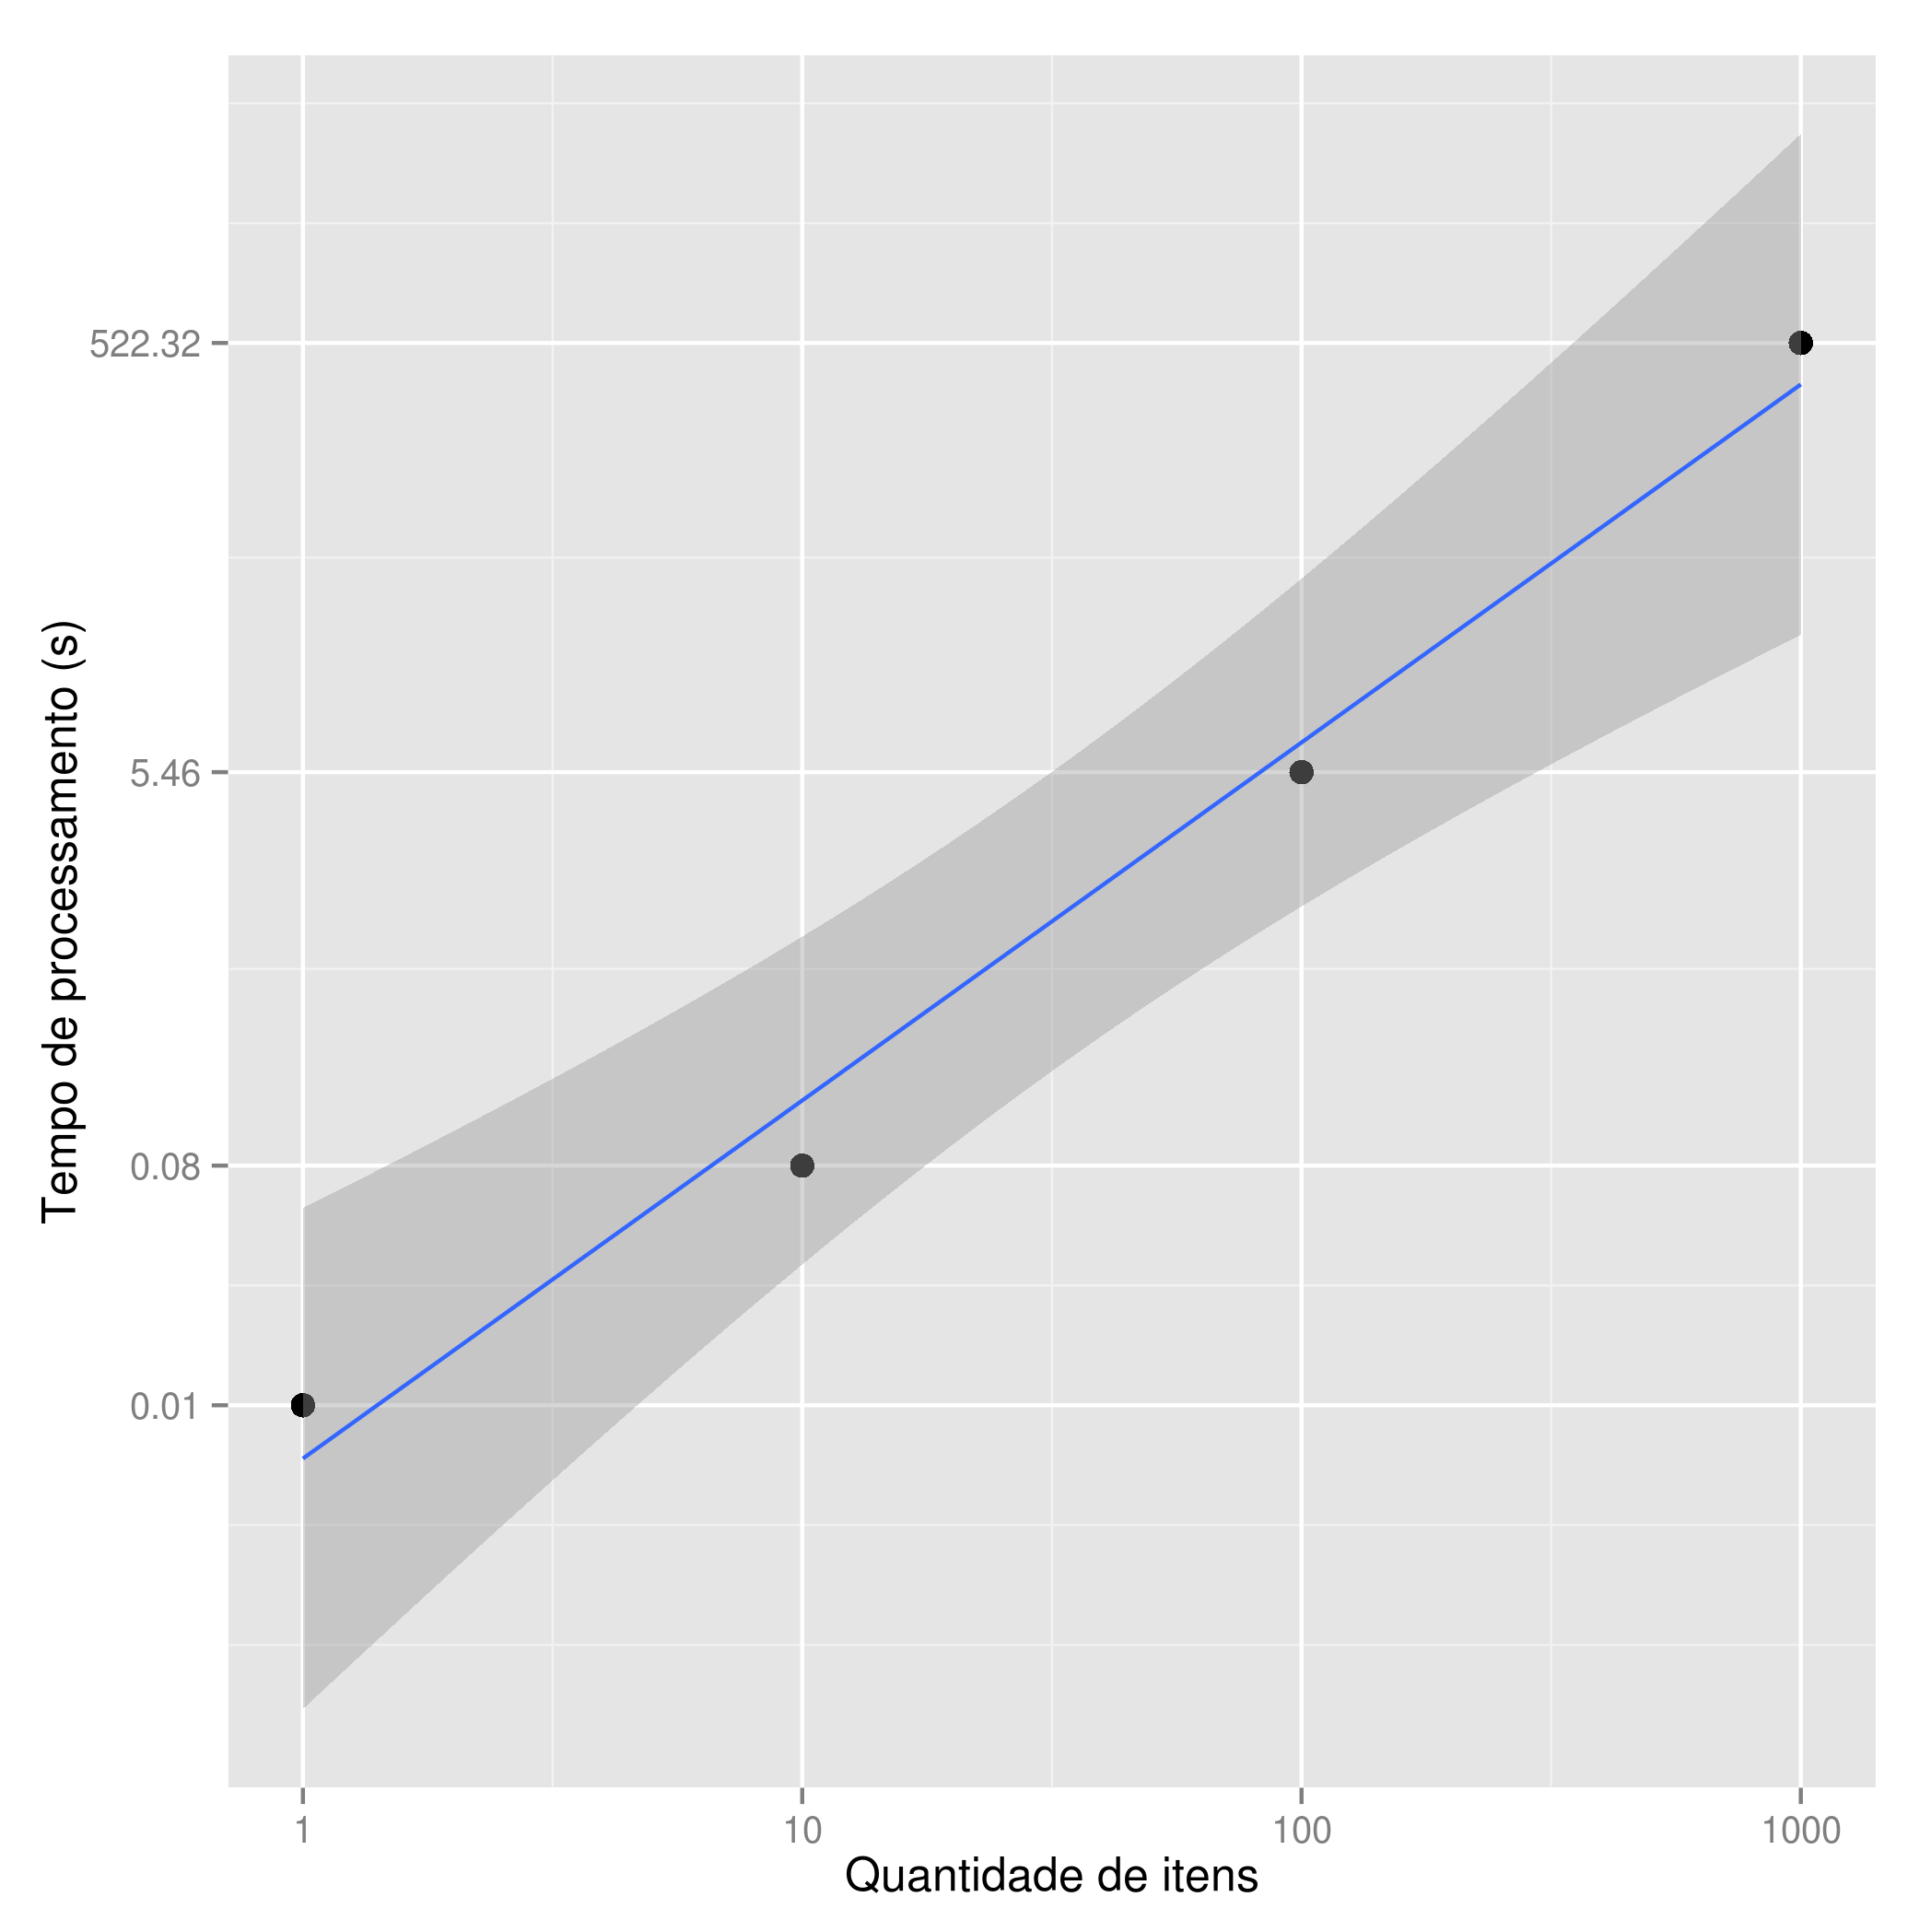
\includegraphics[width=0.9\textwidth]{img/ixt}
    \end{center}
\caption{Tempo de processamento em função do número de itens em $\mathcal{O}\left(n^2\right)$}
\end{figure}
\end{columns}
\end{frame}


\begin{frame}{Resultados}{Aquisição de dados}
\begin{center}
\begin{figure}[ht]
    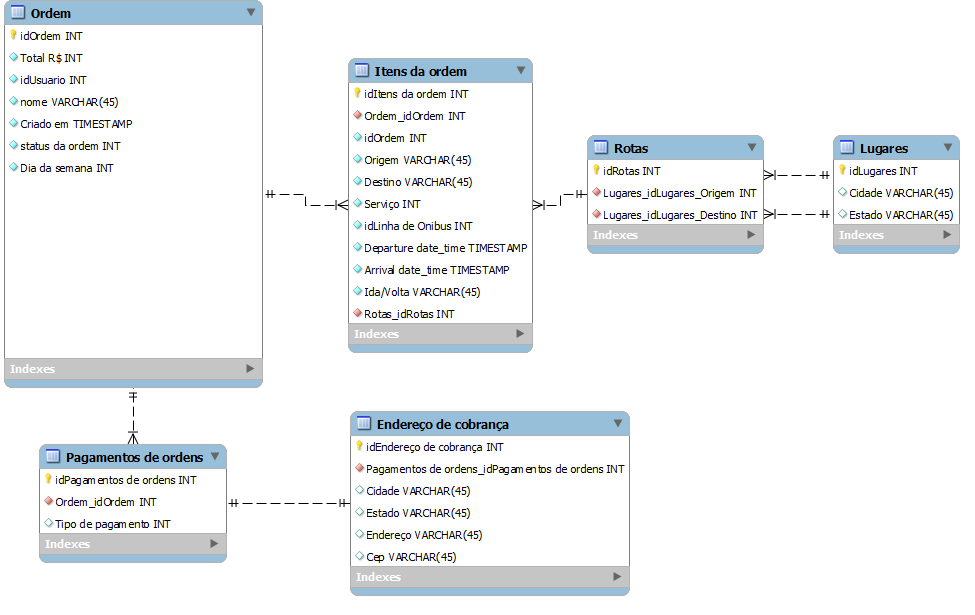
\includegraphics[width=0.8\textwidth]{../img/estrutura-banco-de-dados}
    \caption{Banco de dados de um e-commerce de passagens de ônibus}
    \label{fig:bd-clickbus}
\end{figure}
\end{center}
\end{frame}